\appendices

\section{Experiment 5: Duplication control}
\label{sec:appdup}

The main baseline figure already includes EV-dup, but the broader duplication control remains useful because it shows explicitly that matching the grouped row count by copying the same EV row does not reproduce the grouped-view gain. Cellwise paired comparisons are strongest on Lorenz and NARMA10, where Split beats EV-dup in $9/9$ shot cells, and still favorable on Mackey--Glass, where Split beats EV-dup in $7/9$ shot cells. The weakest Mackey--Glass cells lie at the highest-$\rhoEV$ end of the sweep ($N_{\mathrm{shots}}=10,12,15,18$); from $N_{\mathrm{shots}}=20$ onward, the paired delta is positive and statistically clear in every reported cell.

\begin{figure}[!t]
    \centering
    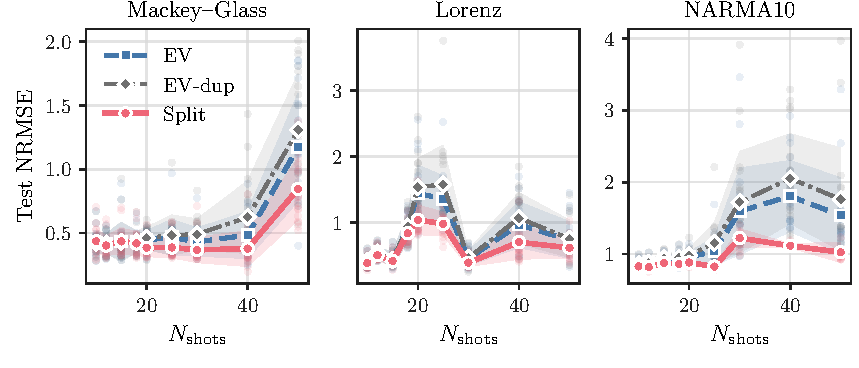
\includegraphics[width=0.98\columnwidth]{experiment_5.pdf}
    \caption{Duplication control from the broader suite. Faint points show matched seeds and the translucent bands show one standard deviation around the mean. Row-count matching by exact duplication is not the same thing as training on several distinct grouped views of the same target.}
    \label{fig:appdup}
\end{figure}

\section{Experiment 3: Larger reservoirs / more qubits}
\label{sec:appmoreqsec}

Figure~\ref{fig:appmoreq} scales the reservoir while keeping the protocol fixed. All three tasks are now shown through $Q=12$ with $20$ seeds per point. The result is stronger and cleaner than in the earlier pilot version: the paired EV-minus-Split delta is positive in all $15/15$ size cells and Wilcoxon-significant in $14/15$. Mackey--Glass is the only weak corner at the smallest reservoir ($Q=4$: $\Delta=0.042\pm0.034$, win-rate $0.65$, Wilcoxon $p=8.3\times10^{-2}$), but from $Q=6$ onward the effect is positive and significant in every Mackey--Glass cell. Lorenz and NARMA10 are favorable throughout the entire sweep.

\begin{figure*}[!t]
    \centering
    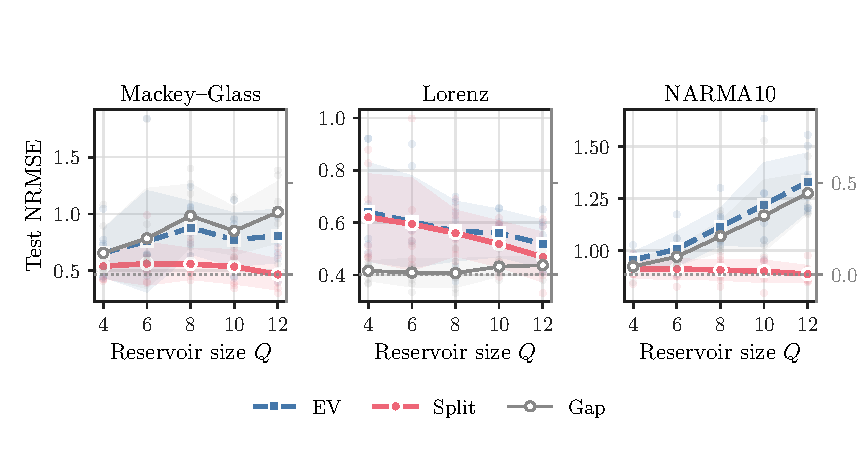
\includegraphics[width=0.98\textwidth]{experiment_3.pdf}
    \caption{Larger-reservoir sweep with $20$ seeds per point. Each panel combines the absolute EV and Split test NRMSE curves with the corresponding EV-minus-Split gap versus reservoir size. The paired EV-minus-Split delta is positive in all shown cells and significant in all but Mackey--Glass at $Q=4$, indicating that the split advantage survives and often strengthens as the feature dimension grows.}
    \label{fig:appmoreq}
\end{figure*}

\section{Experiment 7: Reservoir-architecture ablation}
\label{sec:apparch}

The qubit-count sweep in Figure~\ref{fig:appmoreq} answers the size question, but a reviewer can still ask whether the split gain is tied to one very specific reservoir wiring. To address that directly, we reran the common synthetic operating point at fixed $Q=4$, $N_{\mathrm{shots}}=18$, $\sigma=0$, and $\lambda=10$ across five reservoir variants: ring-CNOT with depths $1$, $2$, and $4$, line-CNOT with depth $1$, and all-to-all CZ with depth $1$. The result is uniform at the sign level: the paired EV-minus-Split delta is positive in all $15/15$ architecture cells and Wilcoxon-significant in $12/15$. The strongest $Q=4$ variant is ring-CNOT depth $2$ on all three tasks, with paired deltas of $\Delta=0.084\pm0.041$ on Mackey--Glass, $\Delta=0.258\pm0.100$ on Lorenz, and $\Delta=0.088\pm0.028$ on NARMA10.

To keep the larger-reservoir follow-up targeted rather than exhaustive, we then ranked the $Q=4$ variants within each dataset by the mean EV-minus-Split gap and reran only the top two variants at $Q=12$ for Mackey--Glass and NARMA10. This targeted extension is again favorable in every tested cell: all $4/4$ paired deltas stay positive and Wilcoxon-significant. On Mackey--Glass, ring-CNOT depth $2$ reaches $\Delta=0.275\pm0.131$ and all-to-all CZ depth $1$ reaches $\Delta=0.150\pm0.078$, both with win-rate $0.875$. On NARMA10, ring-CNOT depth $2$ reaches $\Delta=0.648\pm0.127$ and ring-CNOT depth $4$ reaches $\Delta=0.496\pm0.090$, both with win-rate $1.00$. The conservative readout is therefore not that one single architecture is universally optimal, but that the split advantage is not confined to the default four-qubit ring reservoir used in the main text.

\begin{figure*}[!t]
    \centering
    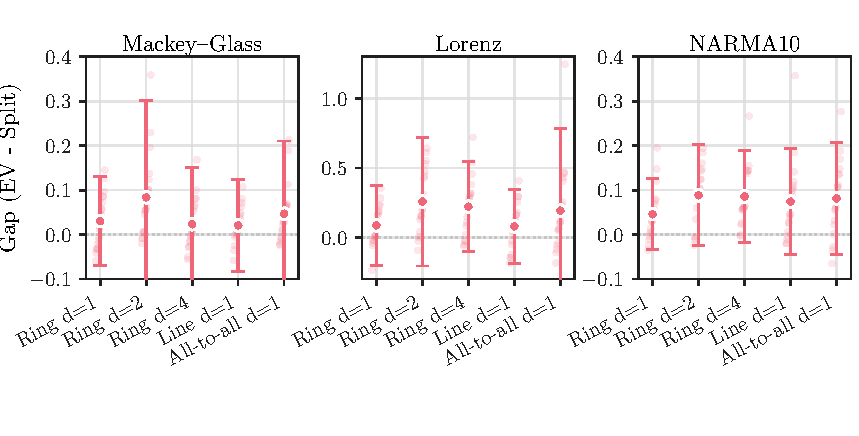
\includegraphics[width=0.98\textwidth]{experiment_7.pdf}
    \caption{Reservoir-architecture ablation at the common operating point ($Q=4$, $N_{\mathrm{shots}}=18$). Faint points show matched seeds; darker markers and error bars show the mean EV-minus-Split gap with one standard deviation. The paired delta remains positive for every reported architecture cell, with the strongest $Q=4$ effect at ring-CNOT depth $2$ on all three datasets.}
    \label{fig:apparch}
\end{figure*}

\section{Closed-form derivation of the warm start}
\label{sec:appkstar}

Define $a:=\sigma_\epsilon^2/\sigma_x^2=1/\mathrm{SNR}_m$. The attenuation factor in Eq.~\eqref{eq:beta0a} is then $\beta_0(k)=k/(k+a)$. The proxy in Eq.~\eqref{eq:proxy} can be written as
\begin{equation}
\mathcal{E}(k)=c_{\mathrm{att}}\left(\frac{a}{k+a}\right)^2 + c_{\mathrm{rows}}\frac{k}{\rhoEV\Nshots}.
\end{equation}
Differentiating and setting the derivative to zero yields
\begin{equation}
(k+a)^3 = \frac{2c_{\mathrm{att}}a^2\rhoEV\Nshots}{c_{\mathrm{rows}}},
\end{equation}
so the continuous minimizer is
\begin{equation}
k_\star^{\mathrm{cont}} = \left(\frac{2c_{\mathrm{att}}}{c_{\mathrm{rows}}}a^2\rhoEV\Nshots\right)^{1/3} - a.
\end{equation}
In practice this value is used only as a warm start: clip it to $[1,\Nshots]$, snap it to the nearest divisor of $\Nshots$, and then validate discretely.

The same derivation also makes the scaling transparent:
\begin{equation}
k_\star \propto \left(\frac{\rhoEV\Nshots}{\mathrm{SNR}_m^2}\right)^{1/3},
\end{equation}
up to the problem-dependent ratio $c_{\mathrm{att}}/c_{\mathrm{rows}}$. Thus larger shot noise pushes toward larger groups, while a more row-limited EV design pushes toward smaller groups.

\section{Implementation details for reproducibility}
\label{sec:apprepro}

\begin{itemize}[leftmargin=*]
    \item Reservoir family: ring-CNOT entanglers with fixed depth unless otherwise stated.
    \item Observables: $\{Z_i,X_i\}_{i=1}^Q$, measured through $\Rsettings=2$ settings.
    \item Features: leaky integrator with rate $\eta=0.2$ and tapped-delay window $L=10$.
    \item Splits: chronological train/validation/test split after a washout of $t_0=30$ time steps; grouping is performed only within split.
    \item Training: ridge regression with protocol-matched validation over divisors of $\Nshots$; features are standardized from the training split only.
    \item Statistics: all non-hardware protocol comparisons are seed-matched. In addition to mean$\pm$standard deviation plots, we report paired mean deltas, 95\% confidence intervals for the paired mean, win-rates, and two-sided Wilcoxon signed-rank $p$-values.
    \item Main synthetic suite: $20$ seeds for representative points, the empirical gap plot, and baseline controls.
    \item Larger-reservoir appendix: $20$ seeds per point for $Q\in\{4,6,8,10,12\}$.
    \item Architecture appendix: $20$ seeds for the full $Q=4$ architecture ablation and $8$ seeds for the targeted $Q=12$ follow-up on Mackey--Glass and NARMA10.
    \item Hardware validation: imported directly from the companion \texttt{ibm\_marrakesh} study with $8$ seeds and no error mitigation.
\end{itemize}
